\section {Этапы компиляции}
\label{sec:steps_of_compilation}

Исполняемый файл получается в результате этапов трансляции и компоновки,
изображённых в \ref{tbl:steps_in_the_production_of_an_executable}

\begin{table}[hc]
	\centering
	\caption{\label{tbl:steps_in_the_production_of_an_executable}Порядок
создания исполняемого файла}
	\begin{tabular}{|l|c|}
	\hline
	 & Исходный текст программы \\
	\hline
	препроцессирование & \\
	\hline
	 & Исходный текст программы \\
	\hline
	компиляция & \\
	\hline
	 & Программа на ассемблере \\
	\hline
	ассемблирование & \\
	\hline
	 & Машинные инструкции \\
	\hline
	компоновка & \\
	\hline
	 & Исполняемый код \\
	\hline
	\end{tabular}
\end{table}

Сначала начинается препроцессирование (макроподстановка), которое подставляет
одни части текста вместо других при помощи системы макросов. Затем исходный код
программы транслируется в команды ассемблера, которые потом конвертируются в
машинные инструкции. Наконец, процесс компоновки (линковки) производит
связывание с элементами операционной системы. Этот процесс включает в себя
добавление библиотеки времени исполнения, которая главным образом состоит из
менеджера памяти.

\subsection {Компиляторы Objective CAML}
\label{subsec:the_objective_caml_compilers}

Детали различных этапов генерации кода компиляторов Objective CAML представлены
таблице \ref{tbl:compilation_stages}. Внутреннее представление кода программы,
сгенерированного компилятором, называется промежуточным языком (ПЯ).

\begin{table}[hc]
	\centering
	\caption{\label{tbl:compilation_stages}Этапы компиляции}
	\begin{tabular}{|l|c|}
	\hline
	 & Последовательность символов \\
	\hline
	лексический анализ & \\
	\hline
	 & Последовательность лексем \\
	\hline
	синтаксический анализ & \\
	\hline
	 & Синтаксическое дерево \\
	\hline
	семантический анализ & \\
	\hline
	 & Аннотированное синтаксическое дерево \\
	\hline
	генерация промежуточного кода & \\
	\hline
	 & Последовательность кода в ПЯ \\
	\hline
	оптимизация промежуточного кода & \\
	\hline
	& Последовательность кода в ПЯ \\
	\hline
	генерация псевдокода & \\
	\hline
	 & Программа на ассемблере\\
	\hline
	\end{tabular}
\end{table}

При помощи лексического анализа из последовательности символов, мы получаем
последовательность лексических элементов (лексем). В основном лексемы
соответствуют целым числам, числам с плавающей запятой, строкам и
идентификаторам. Сообщение \texttt{Illegal character} генерируется на этом
этапе анализа.

Синтаксический анализ создаёт синтаксическое дерево, проверяя при этом
последовательность лексем с точки зрения правил грамматики языка. Сообщение
\texttt{Syntax error} указывает на то, что анализируемая часть кода не
соответствует правилам грамматики.

При семантическом анализе просматривается синтаксическое дерево, здесь нас
интересует другой аспект корректности программы. На этом этапе, в Objective CAML
происходит вывод типа и, если он прошёл удачно, то выводимый тип является самым
общим типом для выражения или объявления. Сообщения об ошибке типа генерируются
на данном этапе. В этот же момент выявляются случаи, в которых тип члена
последовательности отличен от \texttt{unit}. Могут возникать и другие
предупреждения, возникающие на пример во время анализа сопоставления с образцом
(\texttt{pattern matching is not exhaustive}, \texttt{part of pattern matching
will not be used}).

При генерации и оптимизации промежуточного кода не выводится никаких сообщений
об ошибках или предупреждений. Эти этапы манипуляции промежуточными структурами
позволяют факторизовать разработку различных компиляторов Objective CAML.

Генерация исполняемого модуля --- это финальный этап компиляции, который зависит
от компилятора.

\subsection {Описание компилятора байт-кода}

Виртуальная машина Objective CAML называется Zinc (от \enq{Zinc Is Not Caml}).
Она была создана Гзавье Леруа (Xavier Leroy) и описана в (\cite{??}). Это имя
было выбрано, для того чтобы подчеркнуть разницу между первыми реализациями
языка Caml, основанного на виртуальной машине CAM (от Categorical Abstract
Machine, см. \cite{??}).

На рисунке \ref{fig:virtual_machine} изображена виртуальная машина Zinc. В
первой части представлен интерпретатор связанный с библиотекой. Вторая часть
соответствует компилятору, который генерирует байт--код для машины Zinc. Третья
часть содержит библиотеки, идущие вместе с компилятором. Они более подробно
описаны в главе \ref{chpt:libraries}.

\begin{figure}[ch]
	\center{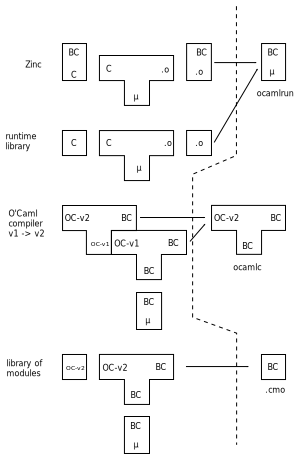
\includegraphics {img/virtual_machine}}
	\caption{\label{fig:virtual_machine}Виртуальная машина}
\end{figure}

Графические символы, используемые на рисунке \ref{fig:virtual_machine}, являются
стандартной нотацией в области компиляторов. Простой блок символизирует файл,
написанный на языке, который указан внутри блока. Двойной блок представляет
интерпретацию одного языка программой, написанной на другом языке. Тройной блок
--- исходный язык компилируется в машинный при помощи компилятора, написанном на
третьем языке. Символы, соответствующие интерпретаторам и компиляторам,
изображены на рисунке
\ref{fig:graphical_notation_for_interpreters_and_compilers}.

\begin{figure}[h]
	\center{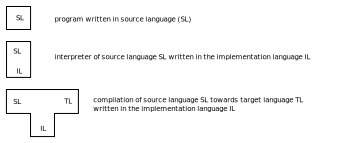
\includegraphics
{img/graphical_notation_for_interpreters_and_compilers}}
	\caption{\label{fig:graphical_notation_for_interpreters_and_compilers}
Символы интерпретаторов и компиляторов}
\end{figure}

Пояснение к рисунку \ref{fig:virtual_machine}:

\begin{itemize}
	\item BC: байт-код машины Zinc

	\item C: код C

	\item .o: объектный файл, зависящий от используемой архитектуры

	\item $\mu$: микропроцессор

	\item OC (v1 или v2): код Objective CAML
\end{itemize}


{\it Замечание}

Основная часть компилятора Objective CAML написана на языке Objective CAML.
Переход с версии v1 на версию v2 изображён на второй части рисунка
\ref{fig:virtual_machine}.
